\documentclass{beamer}
\usetheme{Copenhagen}
\setbeamertemplate{navigation symbols}{}
\usepackage[spanish]{babel}
\usepackage{amsmath, amsthm, amssymb}
\usepackage{graphicx}

\begin{document}

\title{Presentación del buscador Moogle!}
\author{Darío Hernández Cubilla C-113}
\date{17 de julio de 2023}
\maketitle

\section{Modelo Vectorial}

\begin{frame}

\begin{itemize}
    \item<1-> $ \displaystyle tf(w, d) = \dfrac{frecAbs(w, d)}{palabras(d)}$
    \item<2-> $ \displaystyle idf(w, D) = \ln(\frac{ocurrencias(w, D)}{documentos(D)}) $
    \item <3-> Cada dimensión de un vector de documento d representa una palabra w y su coordenada es $ tf(w, d) * idf(w, D)$ 
    \item<4-> $ \displaystyle \cos{\alpha} = \frac{\vec{q}\cdot\vec{d}}{\left\lvert \vec{q} \right\rvert \left\lvert {\vec{d}} \right\rvert }$
             \newline  $\vec{q}$ y $\vec{d}$ representan los vectores de tf-idf de la query q y un documento d del corpus, $\cos{\alpha}$ es su similitud

\end{itemize}

\end{frame}


\section{Utilidades}

\begin{frame}
    \begin{itemize}
        \item<1-> Cacheo
        \item<2-> Corrección Ortográfica
        \item<3-> Búsqueda ampliada con sinónimos
        \item<4-> Snippets 
        \item<5-> Operadores
        \begin{itemize}
            \item<6-> Inclusión: \color{blue}{'\^{}'}
            \item<7-> Exclusión: \color{red}{'!'}
            \item<8-> Aumento de importancia: \color{green}{'*'}
        \end{itemize} 
    \end{itemize}
\end{frame}

\section{Comenzar la búsqueda}

\begin{frame}{Búsqueda de Ejemplo}
    \begin{figure}[h]
        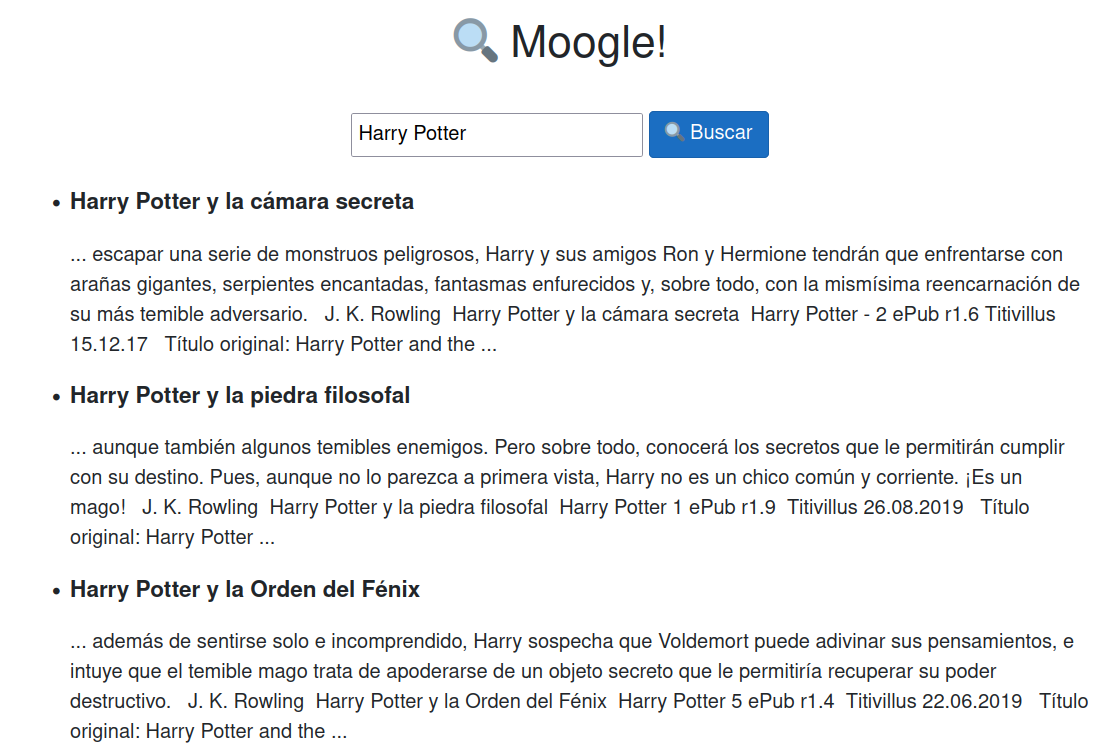
\includegraphics[trim = {0 105  0  0}, clip, width=\textwidth]{sample_search.png}
    \end{figure}
\end{frame}

\section{Operadores}

\begin{frame}{Operador de Exclusión}
    \begin{figure}[h]
        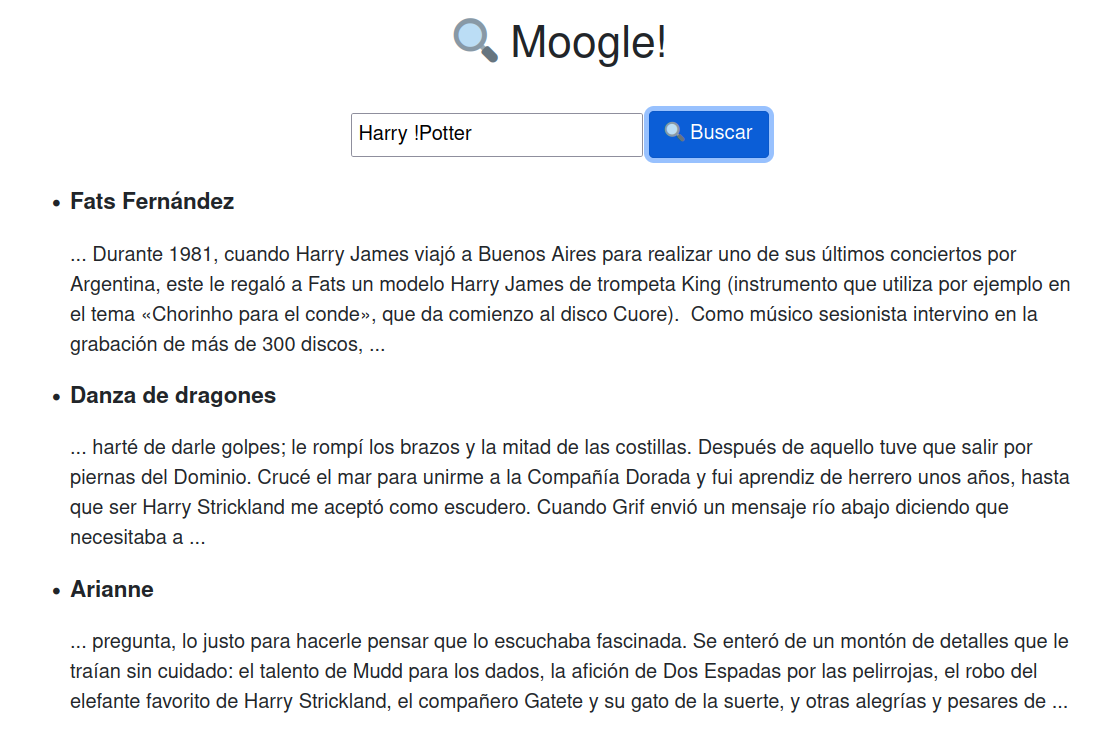
\includegraphics[trim = {0 150  0  0}, clip, width=\textwidth]{ecxlude1.png}
    \end{figure}
\end{frame}

\begin{frame}{Operador de Inclusión, Original}
    \begin{figure}[h]
        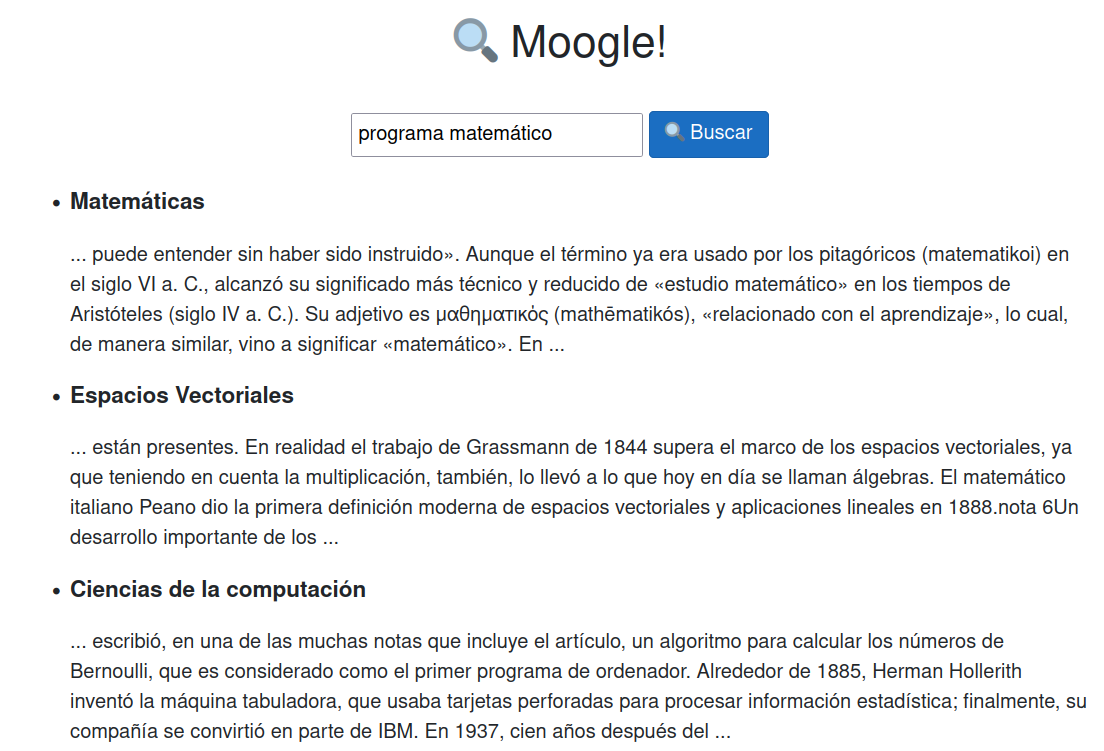
\includegraphics[trim = {0 105  0  0}, clip, width=\textwidth]{include1.png}
    \end{figure}
\end{frame}

\begin{frame}{Operador de Inclusión, Modificado}
    \begin{figure}[h]
        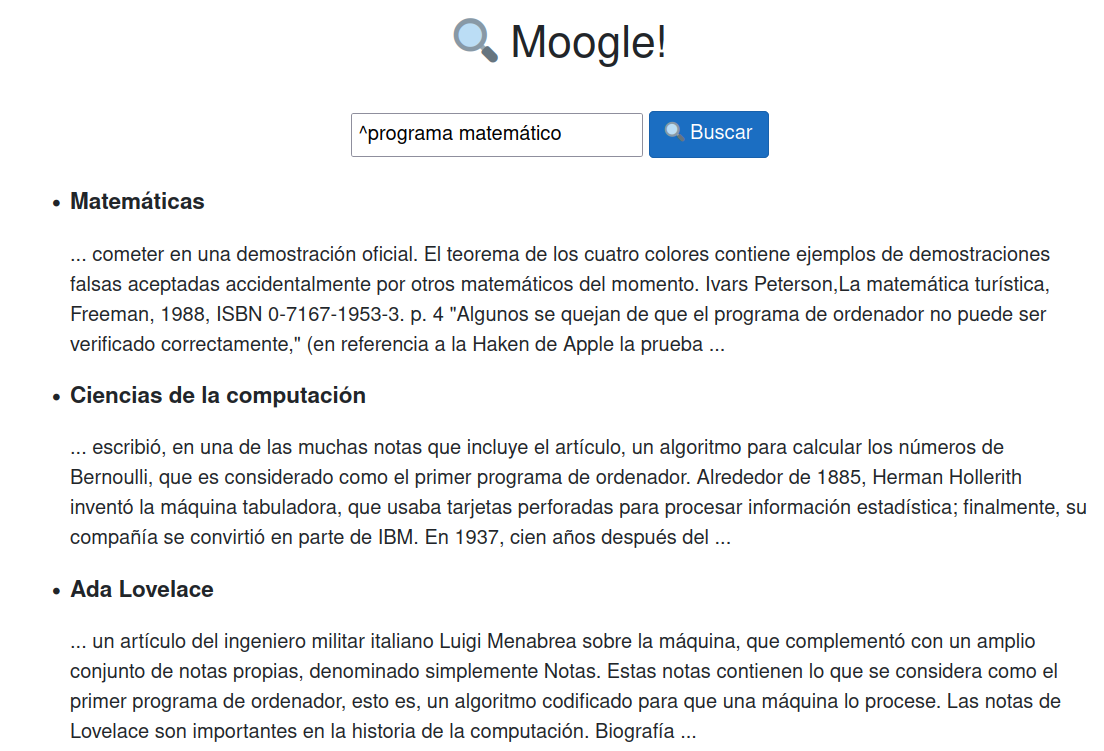
\includegraphics[trim = {0 105  0  0}, clip, width=\textwidth]{include2.png}
    \end{figure}
\end{frame}


\begin{frame}{Operador de aumento de importancia, Original}
    \begin{figure}
        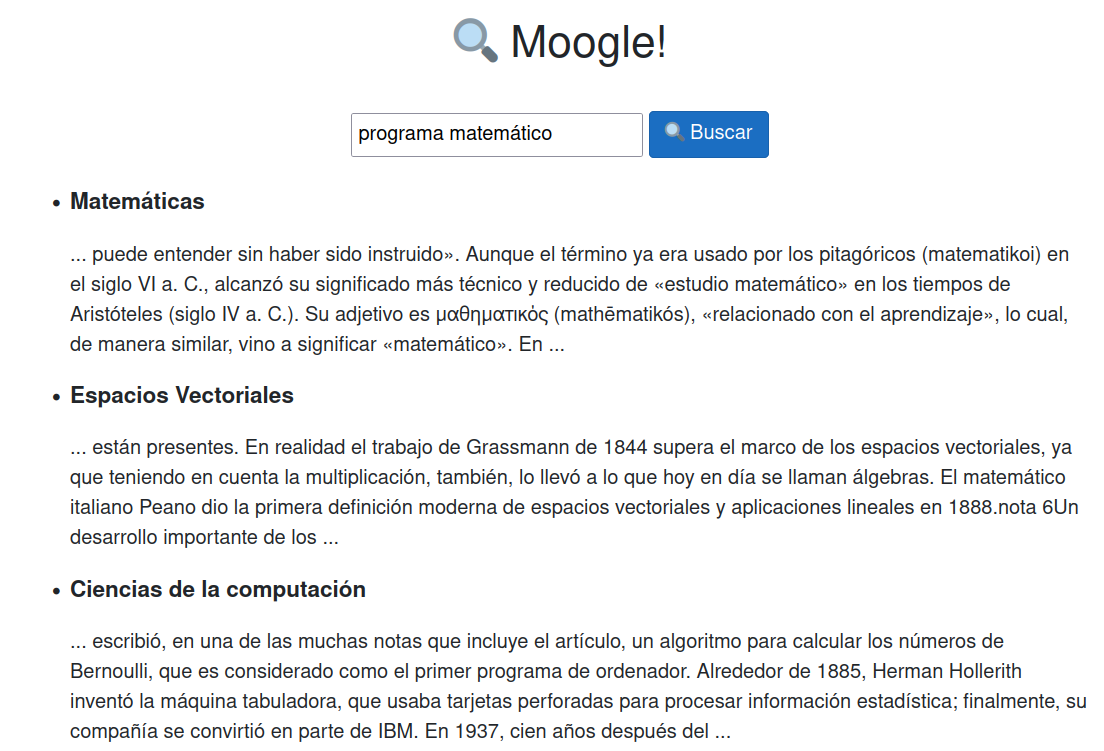
\includegraphics[trim = {0 105  0  0}, clip, width=\textwidth]{include1.png}
    \end{figure}
\end{frame}

\begin{frame}{Operador de aumento de importancia, Modificado}
    \begin{figure}
        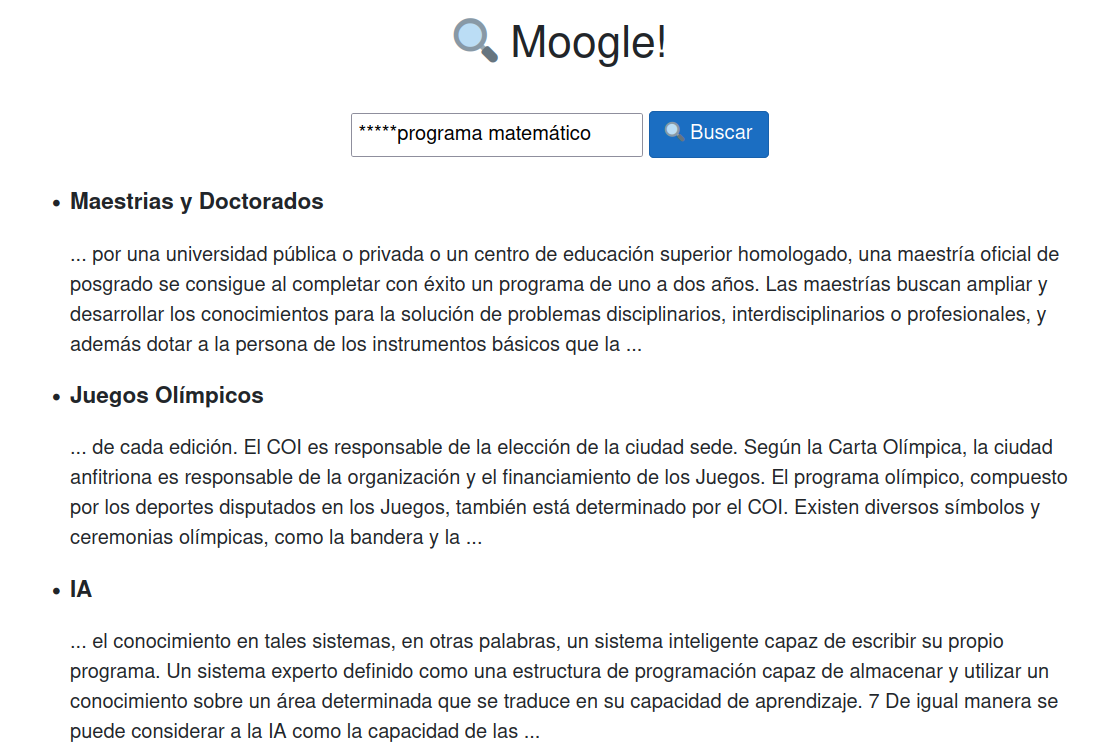
\includegraphics[trim = {0 105  0  0}, clip, width=\textwidth]{asterisk2.png}
    \end{figure}
\end{frame}

\section{Corrección Ortográfica}

\begin{frame}{Corrección Ortográfica}
    \begin{figure}
        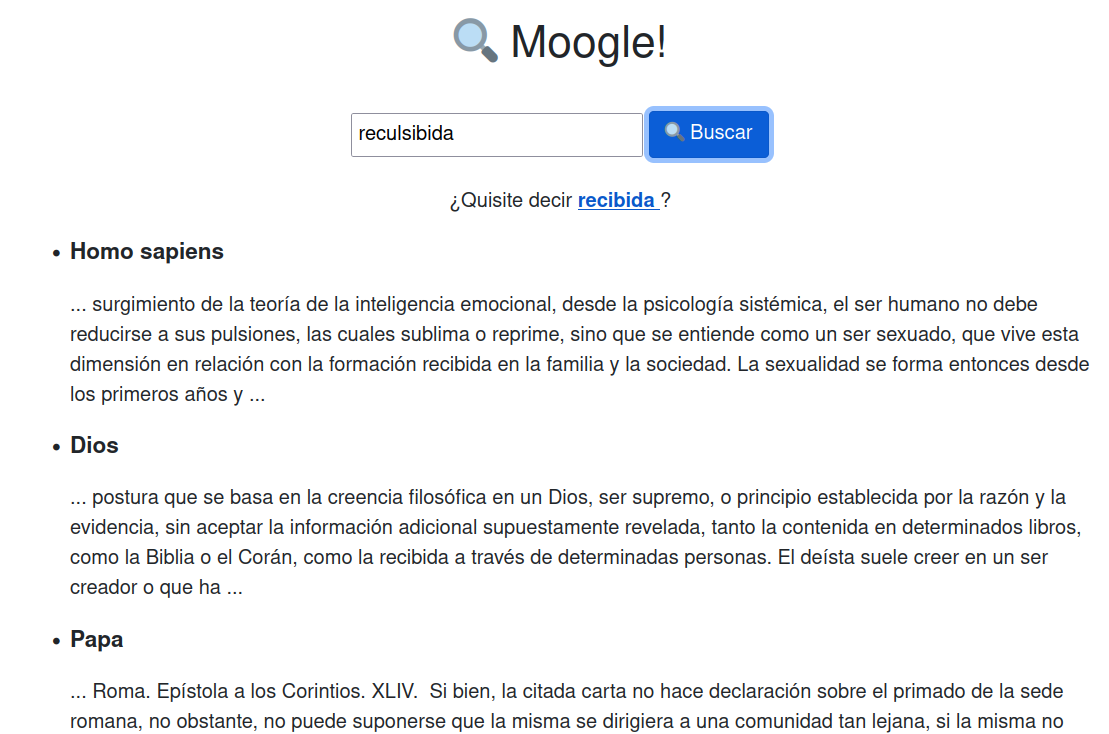
\includegraphics[trim = {0 105  0  0}, clip, width=\textwidth]{correction.png}
    \end{figure}
\end{frame}


\section{Snippet}

\begin{frame}{Snippet}
    \begin{figure}
        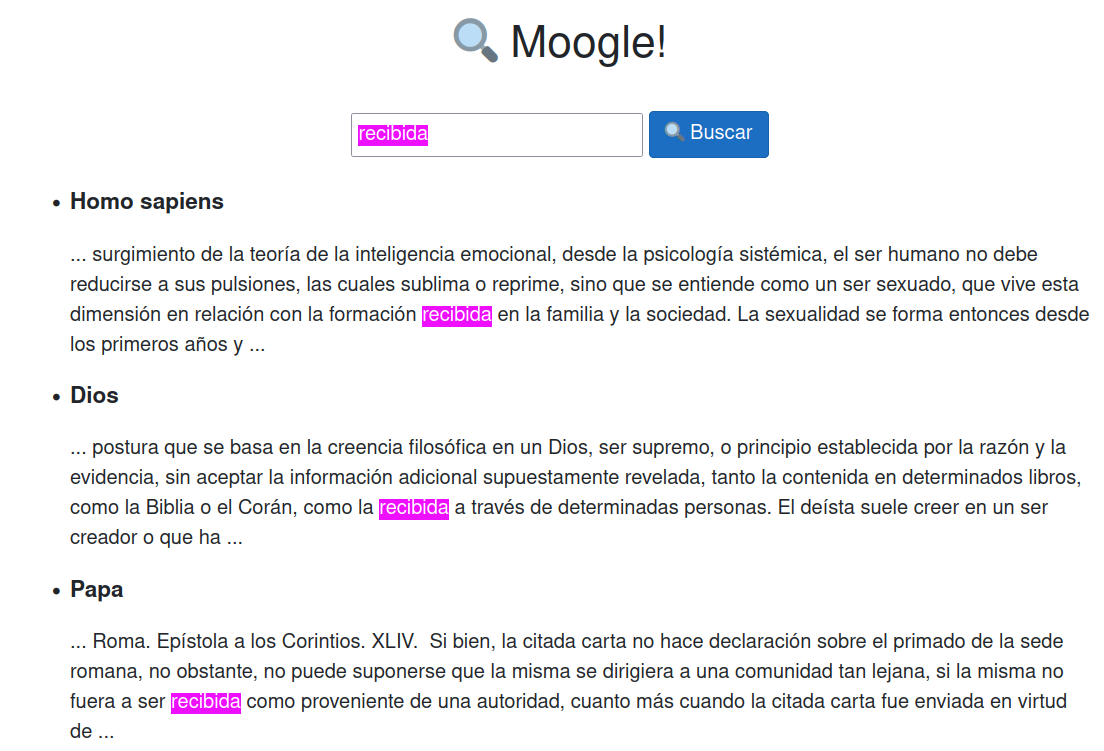
\includegraphics[trim = {0 105  0  0}, clip, width=\textwidth]{snippet.png}
    \end{figure}
\end{frame}



\end{document}

